\documentclass{article}
\usepackage{pgfplots}

\pgfplotsset{compat=1.3}
\usepgfplotslibrary{patchplots}

\begin{document}
\thispagestyle{empty}

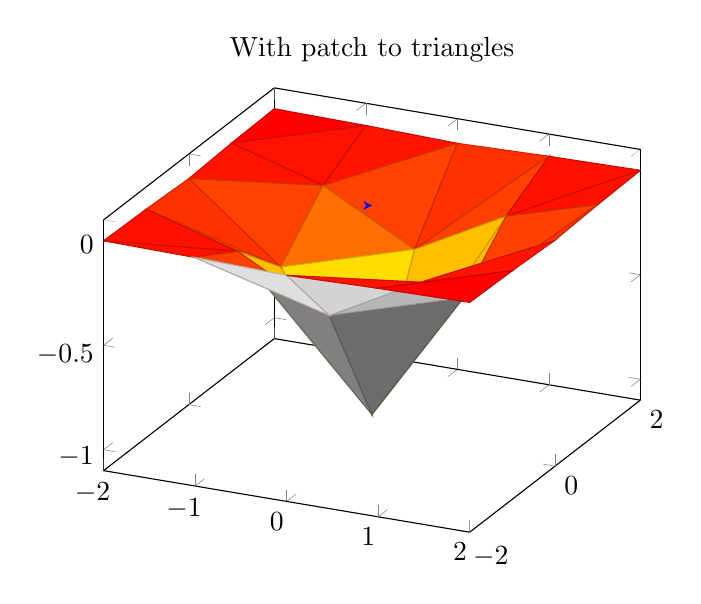
\begin{tikzpicture}
%\tracingmacros=2 \tracingcommands=2
	\begin{axis}[domain=-2:2,
		title=With patch to triangles,
		mesh/interior colormap name={hot},
		colormap/blackwhite,
		samples=5,
		%nodes near coords=\coordindex,
		patch to triangles,
		%mesh/show normals,
	]
	\addplot3[surf] {-exp(-x^2-y^2)};
	\draw[-stealth,blue] (axis cs:0,0,0)  \pgfextra{\pgfpathlineto{\pgfpointadd{\pgfplotspointaxisxyz000}{\pgfplotspointviewdir}}};
	\end{axis}
\end{tikzpicture}

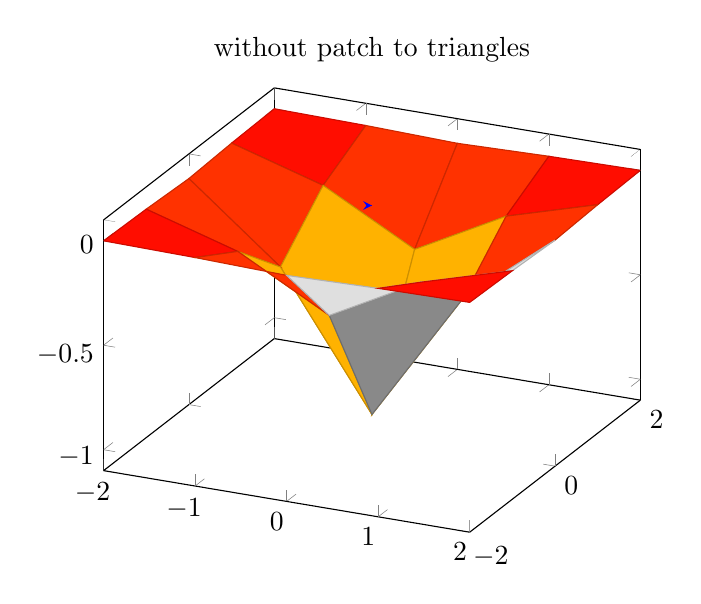
\begin{tikzpicture}
%\tracingmacros=2 \tracingcommands=2
	\begin{axis}[domain=-2:2,
		title=without patch to triangles,
		mesh/interior colormap name={hot},
		colormap/blackwhite,
		samples=5,
		%disabledatascaling,
		%nodes near coords=\coordindex,
		%patch to triangles,
		%mesh/show normals,
	]
	\addplot3[surf] {-exp(-x^2-y^2)};
	\draw[-stealth,blue] (axis cs:0,0,0)  \pgfextra{\pgfpathlineto{\pgfpointadd{\pgfplotspointaxisxyz000}{\pgfplotspointviewdir}}};
	\end{axis}
\end{tikzpicture}


\end{document}

